\chapter{Results}
\label{ch:results}

\section{Parameter analysis}

\subsection{Point cloud voxelization}
\begin{table}[h]
    \centering
    \begin{tabular}{|c|c|c|c|c|c|c|c|c|}
        \hline
        \textbf{Voxel} & \textbf{Median}   & \textbf{ATE}    & \textbf{ATE}  & \textbf{Final } & \textbf{Final} & \textbf{Avg.} & \textbf{Avg.}   & \textbf{Avg.}  \\
        \textbf{Size}  & \textbf{Duration} & \textbf{Trans.} & \textbf{Rot.} & \textbf{Error}  & \textbf{Error} & \textbf{RMSE} & \textbf{Corr.}  & \textbf{Corr.} \\
                       &                   & \textbf{}       & \textbf{}     & \textbf{Trans.} & \textbf{Rot.}  & \textbf{}     & \textbf{Trans.} & \textbf{Rot.}  \\
        \hline
        \hline
        0.1            & 0.2984            & 1.0569          & 0.0265        & 2.5337          & 0.0467         & 0.0555        & 0.0080          & 0.0010         \\
        0.2            & 0.1684            & 1.1386          & 0.0283        & 2.7607          & 0.0511         & 0.0868        & 0.0210          & 0.0024         \\
        0.3            & 0.1586            & 1.2803          & 0.0317        & 3.0500          & 0.0542         & 0.1206        & 0.0351          & 0.0040         \\
        0.4            & 0.1589            & 1.4727          & 0.0384        & 3.5078          & 0.0659         & 0.1545        & 0.0519          & 0.0055         \\
        0.5            & 0.1603            & 1.2081          & 0.0324        & 2.9164          & 0.0568         & 0.1876        & 0.0819          & 0.0077         \\
        0.6            & 0.1635            & 1.6171          & 0.0444        & 3.7190          & 0.0677         & 0.2186        & 0.1069          & 0.0116         \\
        \hline
    \end{tabular}
    \caption{Metrics for varying voxel sizes.}
    \label{tab:voxel_metrics}
\end{table}

\begin{figure}[h]
    \centering
    \subcaptionbox{Distribution of point entropies.}{
        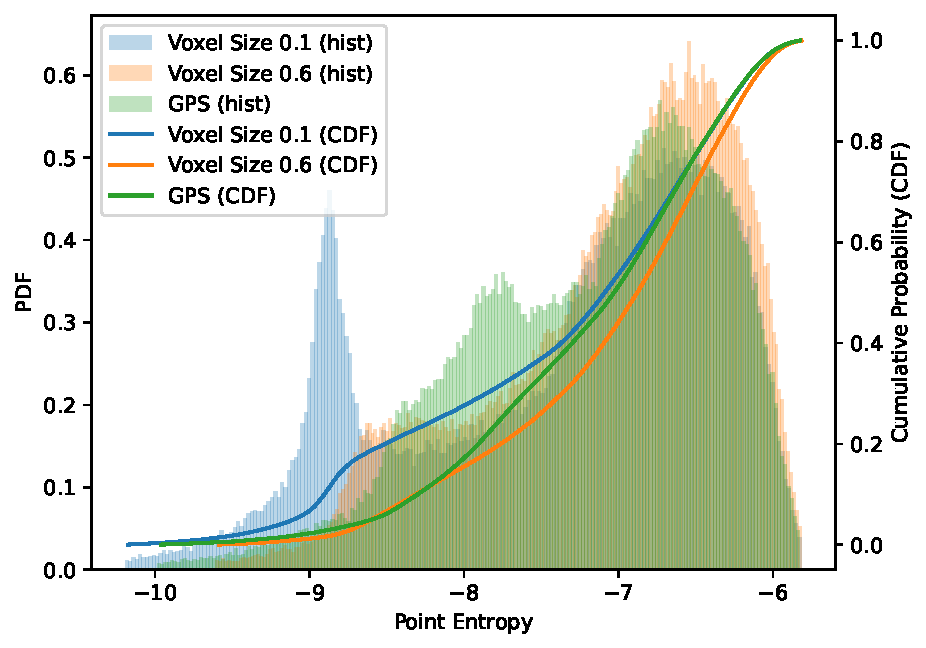
\includegraphics[width=0.45\linewidth]{images/voxel-size-entropy.pdf}
    }
    \hspace{1pt}
    \subcaptionbox{Visual comparison. }{
        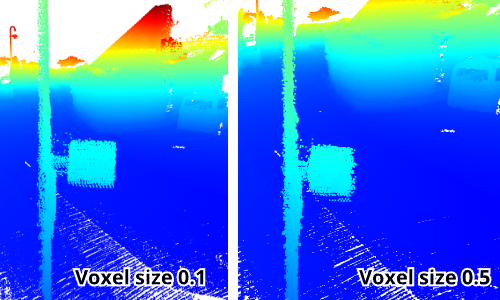
\includegraphics[width=0.47\linewidth]{images/voxel-size-comp.png}
    }
    \caption[Voxel size effect on map quality]{Voxel size effect on map quality.}
    \label{fig:gicp-corrections}
\end{figure}



% \begin{figure}[h]
%     \centering
%     \subcaptionbox{Translation corrections.}{
%         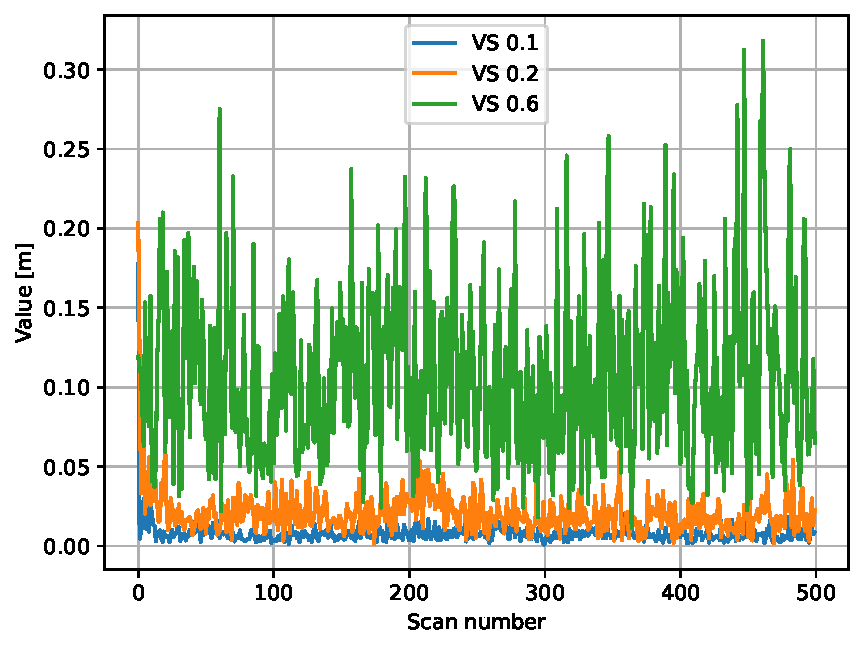
\includegraphics[width=0.46\linewidth]{images/gicp_corrections_trans.pdf}
%     }
%     \hspace{1pt}
%     \subcaptionbox{Rotation corrections.}{
%         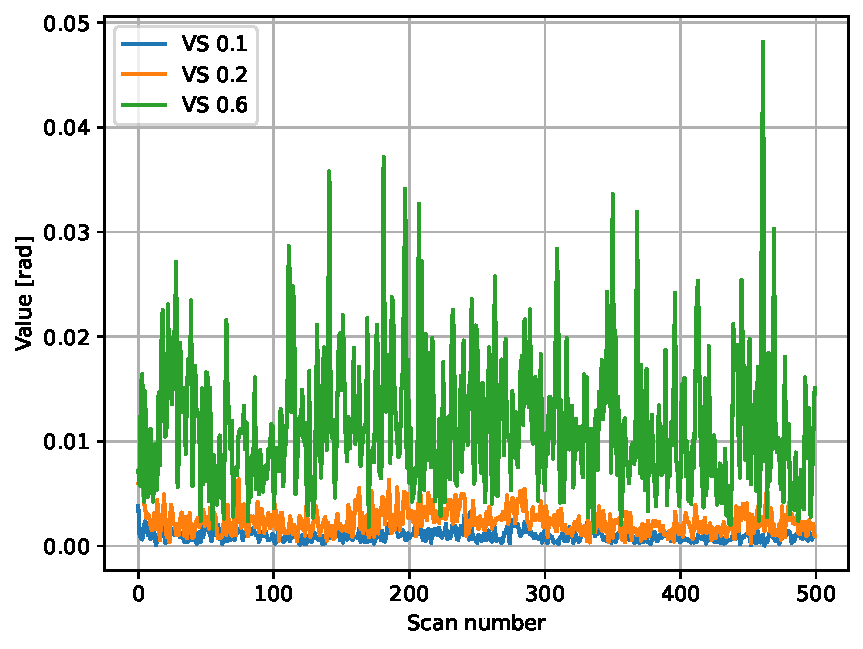
\includegraphics[width=0.45\linewidth]{images/gicp_corrections_rot.pdf}
%     }
%     \caption[]{
%     }
%     \label{fig:gicp-corrections}
% \end{figure}

\subsection{Local map size}
%% how do the results change, depending on the number of previous scans
% test with 1, 2, 5, 10, 15


\begin{table}[h]
    \centering
    \begin{tabular}{ccccccccc}
        \hline
        \textbf{Map}  & \textbf{Median}   & \textbf{ATE}    & \textbf{ATE}  & \textbf{Final } & \textbf{Final} & \textbf{Avg.} & \textbf{Avg.}   & \textbf{Avg.}  \\
        \textbf{Size} & \textbf{Duration} & \textbf{Trans.} & \textbf{Rot.} & \textbf{Error}  & \textbf{Error} & \textbf{RMSE} & \textbf{Corr.}  & \textbf{Corr.} \\
                      &                   & \textbf{}       & \textbf{}     & \textbf{Trans.} & \textbf{Rot.}  & \textbf{}     & \textbf{Trans.} & \textbf{Rot.}  \\
        \hline \hline
        1             & 0.2349            & 4.0721          & 0.1376        & 10.2891         & 0.2603         & 0.0940        & 0.0366          & 0.0021         \\
        2             & 0.2308            & 3.5227          & 0.1186        & 9.1949          & 0.2318         & 0.0818        & 0.0171          & 0.0016         \\
        5             & 0.2632            & 1.4967          & 0.0410        & 3.6849          & 0.0734         & 0.0615        & 0.0094          & 0.0011         \\
        10            & 0.2962            & 1.0569          & 0.0265        & 2.5337          & 0.0467         & 0.0555        & 0.0080          & 0.0010         \\
        15            & 0.3242            & 0.9653          & 0.0238        & 2.2848          & 0.0415         & 0.0540        & 0.0076          & 0.0010         \\
        25            & 0.3984            & 0.9182          & 0.0223        & 2.1504          & 0.0384         & 0.0531        & 0.0079          & 0.0011         \\
        \hline
    \end{tabular}
    \caption{Metrics for varying map sizes.}
    \label{tab:map_sizes}
\end{table}

\subsection{Registration strategy}
%% how do the results change, depending on whether we use GICP or not


\section{Odometry evaluation}

\section{Mapping evaluation}

\section{KITTI results}

% Things worth mentioning
% - execution time